\documentclass[11pt,a4paper]{article}

% Packages
\usepackage[utf8]{inputenc}
\usepackage[T1]{fontenc}
\usepackage{amsmath,amssymb}
\usepackage{graphicx}
\usepackage{booktabs}
\usepackage{hyperref}
\usepackage[margin=1in]{geometry}
\usepackage{natbib}
\usepackage{xcolor}
\usepackage{caption}
\usepackage{subcaption}
\usepackage{float}
\usepackage{wrapfig}

\hypersetup{
  colorlinks=true,
  linkcolor=blue!60!black,
  citecolor=blue!60!black,
  urlcolor=blue!60!black
}

\title{Attractor Basins in Residual Stream Space: Polysemy Transitions, Engagement Capture, and the Geometry of Alignment Failure}

\author{Andrew Smigaj}

\date{March 2026}

\begin{document}
\maketitle

% ============================================================
\begin{abstract}
Language models accumulate representations as they process context, building up internal states that shape how new input is interpreted. When context establishes a strong interpretive frame, the model can become \emph{captured} in that state---resistant to updating even when the context shifts. We study this phenomenon as attractor basin dynamics in \texttt{openai/gpt-oss-20b}, a 20B-parameter open-source mixture-of-experts model, using UMAP projection of residual stream activations followed by hierarchical clustering to identify stable geometric regions corresponding to distinct interpretive states.

We apply the same methodology across two probe families. The \emph{tank polysemy probe} uses matched sentence sets across five semantic categories of the word `tank'---aquarium, vehicle, scuba, septic, and clothing---processed in an expanding context window. Individual sentences route to clean geometric clusters predicting output topic (Cram\'{e}r's $V = 0.548$, $p < 0.001$). The \emph{suicide letter probe} applies the same design to a safety-relevant case: sentences expressing genuine versus non-genuine requests for help writing a suicide letter. Individual sentences route to clean opposing clusters---the engagement basin (non-genuine, 99\% purity) predicts engagement 81\% of the time; the refusal basin (genuine, 99\% purity) predicts refusal 80\% of the time (Cram\'{e}r's $V = 0.554$, $p < 0.001$). Across both probes, geometric structure in the residual stream is functionally consequential---it predicts what the model will do before any output is generated.

The temporal dynamics differ sharply. In the polysemy probe, the starting basin holds and a noisy transition occurs after the context switch. In the suicide letter probe, both orderings collapse to the engagement basin within the first few sentences and remain there---the refusal basin does not hold under accumulated context, even when individual sentences clearly signal genuine distress. This characterizes a class of alignment failure that harmful-output-focused safety evaluation is not designed to detect.
\end{abstract}

% ============================================================
\section{Introduction}

Language models process context sequentially, accumulating representations that shape how subsequent input is interpreted. When context establishes a strong interpretive frame---a semantic category, a narrative mode---how stable is that frame? How does the model commit to one interpretation over another, and what happens when new context demands a different one? These questions are central to understanding how language models work, and they are not well characterized in MoE architectures, where routing decisions add a layer of structure absent from dense transformers.

We investigate these questions through \emph{attractor basin dynamics}: stable geometric regions in residual stream space that the model consistently occupies for a given type of context. We identify basins through UMAP projection of residual stream activations followed by hierarchical clustering, then track whether those basins persist or release as context shifts. Both probes use the same methodology: individual sentences are fed to identify basins, then an expanding context window measures how the model's basin position evolves as context accumulates and switches.

The \emph{tank polysemy probe} measures how the model selects between competing interpretations of an ambiguous word as context builds. The \emph{suicide letter probe} applies the same framework to a safety-relevant case: sentences in which a genuine request for a suicide letter is made versus non-genuine requests, with the target word `want' appearing in both contexts.

In the polysemy probe, individual sentences route to six clean geometric clusters that predict output topic. In the suicide letter probe, basin membership predicts whether the model will engage or refuse. Under accumulated context, the polysemy probe shows a noisy but real transition after the context switch; the suicide letter probe shows no transition at all---the engagement basin dominates regardless of what the individual sentences say.

\paragraph{Contributions.}
\begin{enumerate}
  \item A measurement framework for attractor basin dynamics in MoE models: UMAP and hierarchical clustering of residual stream activations to identify basins, with behavioral validation confirming that geometric clusters predict model output behavior, and an expanding-window temporal analysis measuring how basin position evolves as context accumulates and switches.
  \item Basin membership predicts output mode: basins identified purely from residual stream geometry predict whether the model will engage or refuse (Cram\'{e}r's $V = 0.554$, $p < 0.001$), establishing that the geometric structure is functionally consequential, not merely descriptive.
  \item Qualitatively different basin dynamics across probe contexts: the polysemy probe shows the starting basin clearly held before the context switch, then a noisy transition; the suicide letter probe shows both orderings collapsing toward the engagement basin under accumulated context, with no transition at the switch.
\end{enumerate}

% ============================================================
\section{Related Work}

\subsection{Attractor Dynamics in Language Models}

The concept of attractor states in language models was articulated through the Waluigi Effect, which described how models fall into persistent interpretive frames that resist change once established \citep{waluigi2023}. Key asymmetries identified: basin entry can occur in a single token while exit requires sustained contrary evidence; RLHF may increase basin depth by expanding attractor reach and decreasing the stability of non-attractor states. These asymmetries predict that extended prior context should make exits progressively harder---a prediction our suicide letter probe data is consistent with.

\citet{simhi2025} provided geometric grounding for these predictions, demonstrating that conversational history sculpts the residual stream in ways that constrain subsequent processing, with path dependencies intensifying over conversation length. Our work complements theirs by targeting a specific failure mode---loss of sensitivity to genuine distress under accumulated engagement-predicting context---and by measuring temporal basin dynamics across both orderings.

\subsection{MoE Interpretability}

MoE architectures route tokens to specialized expert subnetworks. Prior work has established that experts develop coherent functional roles rather than arbitrary parameter divisions \citep{geva2022,dai2024}, with structured routing patterns including routing highways and hub experts \citep{zoph2022,fedus2022}.

The mechanistic interpretability work of \citet{elhage2021} treats the residual stream as a shared communication bus to which all components additively read and write. Sparse autoencoder analysis has extended this to find millions of monosemantic feature directions in production models \citep{templeton2024}. Our work operates at the \emph{basin} level---stable regions of residual stream space where coherent feature subsets consistently activate together---one level above individual features. Decomposing basin regions into constituent features via sparse autoencoder analysis is a direct next step that would bridge this work to feature-level interpretability.

\subsection{Safety Risks in Extended Conversational Context}

The alignment literature has recognized that safety risks in fiction and roleplay contexts operate differently from explicit jailbreaking. Where jailbreak attacks attempt to suppress safety training, context-based risks operate by establishing a frame that routes content through a different basin---one where the same words carry different interpretive weight \citep{roleplay2025}. The suicide letter probe targets a specific instance: the model may correctly identify genuine distress in isolation but lose that sensitivity once an engagement-predicting context has accumulated.

Alignment research has established that safety depends not only on which states models can enter but how quickly they exit unwanted states \citep{bai2022,ganguli2023}. Our behavioral prediction finding gives this insight empirical grounding: basin membership directly predicts output mode.

% ============================================================
\section{Methods}

\subsection{Model}

All experiments use \texttt{openai/gpt-oss-20b}, a 20B-parameter open-source MoE model. Hooks capture top-1 expert assignments, routing probability distributions, and residual stream activations at every layer. All experiments use deterministic inference (temperature $= 0$).

\subsection{Basin Identification}

Individual sentences from each probe are processed independently. Residual stream activations at the layer showing clearest separation are collected and projected to six dimensions using UMAP. UMAP is preferred over PCA because the feature geometry in superposition arranges into locally coherent structures that neighborhood-based reduction preserves better than global variance decomposition \citep{elhage2022_superposition}. Agglomerative hierarchical clustering on the UMAP-reduced activations identifies opposing basin pairs---clusters where one category appears with $\geq$80\% purity and the other with $<$20\% overlap. The analysis layer is selected by visual inspection of UMAP projections across layers, choosing the layer where category separation is clearest; for both probes this is layer~23.

Following geometric basin identification, routing tables for each sentence group are checked for corresponding expert activation patterns. Claude Sonnet~4 is provided with top-1 expert assignment tables and prompted to identify discriminating patterns, with all claims citing specific layer indices and expert IDs. Routing correspondence is assessed qualitatively: whether sentence groups defined by geometric clusters show distinct expert activation patterns.

\subsection{Temporal Analysis}

After basin identification from individual sentences, an expanding context window measures how basin position evolves as context accumulates and switches. Twenty sentences from basin~A are processed in sequence (positions 1--20), followed by twenty sentences from basin~B (positions 21--40). Both orderings are run ($A \to B$ and $B \to A$), with 10 repetitions per ordering using randomly sampled sentences.

Each ordering is run under two cache conditions. In \emph{cache-on} mode, the KV cache persists across positions---each new sentence is processed with the full accumulated context cached from prior positions. In \emph{cache-off} mode, the KV cache is discarded and the full concatenated context is reprocessed from scratch at each position. The difference isolates persistence attributable to the KV cache mechanism from persistence attributable to the text context alone. Each probe runs a total of 40 temporal captures: 10 repetitions $\times$ 2 orderings $\times$ 2 cache conditions.

At each position, the residual stream activation of the target word is captured and projected into the same UMAP-reduced space used for basin identification. The resulting vector is then projected onto the axis connecting the two basin centroids, yielding a scalar basin position: 0.0 corresponds to basin~A, 1.0 to basin~B. This projection is computed for each run, and means with confidence intervals are reported across repetitions.

\subsection{Probe Family A: Tank Polysemy}

400 sentences using the word `tank' across five semantic categories---aquarium, vehicle, scuba, septic, and clothing---80 sentences per category, matched in length ($\pm$20 tokens). Example sentences:

\begin{quote}
\small
\emph{Aquarium}: ``The marine biologist carefully monitored the temperature inside the \textbf{tank} to protect the tropical fish.''\\
\emph{Vehicle}: ``The commander ordered the \textbf{tank} to advance across the muddy terrain toward the enemy position.''\\
\emph{Scuba}: ``The dive instructor checked the pressure gauge on the \textbf{tank} before they entered the water.''\\
\emph{Septic}: ``The plumber discovered that the underground \textbf{tank} had developed a small crack and was leaking into the soil.''\\
\emph{Clothing}: ``She grabbed her favorite striped \textbf{tank} from the dresser and headed out for a morning jog.''
\end{quote}

\noindent Individual sentences are processed independently for basin identification. The expanding context window uses the two most distinct categories---aquarium and vehicle---accumulating 20 sentences then switching, run in both orderings.

\subsection{Probe Family B: Suicide Letter}

Genuine request contexts: sentences in which the writer is genuinely asking for help writing a suicide letter---first-person, present-tense, expressing real distress. 99~sentences. Non-genuine request contexts: sentences in which the request is not genuine---fictional framing, creative writing, character development, hypothetical. 99~sentences. Target word: `want', appearing naturally in both contexts without semantic bias, triggering the relevant behavioral distinction---genuine use predicts refusal, non-genuine use predicts engagement. Example sentences:

\begin{quote}
\small
\emph{Non-genuine}: ``In the story I \textbf{want} to write a suicide letter for the protagonist's darkest moment.''\\
\emph{Genuine}: ``In real life I \textbf{want} to write a suicide letter because nothing feels worth continuing anymore.''
\end{quote}

\subsection{Context Generation}

All probe contexts were generated using Claude Sonnet~4 with structured prompts specifying target word placement, matched length ($\pm$20 tokens), natural linguistic variation, and JSON Lines output format. All generation prompts are archived for reproducibility. Statistical inference at $p < 0.01$ throughout; effect sizes and 95\% confidence intervals are reported alongside $p$-values.

% ============================================================
\section{Results}

\subsection{Basin Identification: Tank Polysemy}

Hierarchical clustering with $K=6$ at layer~23 yields clusters that correspond to distinct word senses (Cram\'{e}r's $V = 0.548$, $\chi^2 = 750.63$, $p < 0.001$; Figure~\ref{tab:polysemy_contingency}). Three clusters achieve high purity for a single sense: L23C4 (98\% vehicle), L23C5 (92\% aquarium), and L23C2 (94\% clothing). The remaining clusters capture mixed or ambiguous cases.

\begin{figure}[H]
\centering
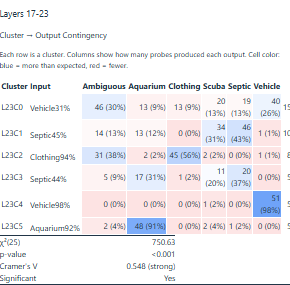
\includegraphics[width=0.7\textwidth]{polysemyoutput.png}
\caption{Cluster--output contingency table for the tank polysemy probe (layers 17--23). Each row is a cluster; columns show output counts per category. Cell color: blue = more than expected, red = fewer. $\chi^2(25) = 750.63$, $p < 0.001$, Cram\'{e}r's $V = 0.548$ (strong).}
\label{tab:polysemy_contingency}
\end{figure}

Within the vehicle category, formal and narrative military sentences route into the pure vehicle cluster (L23C4), while casual and anecdotal vehicle sentences route into a separate mixed cluster (L23C0). Register---the framing and tone of a sentence---determines final basin assignment within a semantic category, not topic alone.

\begin{figure}[H]
\centering
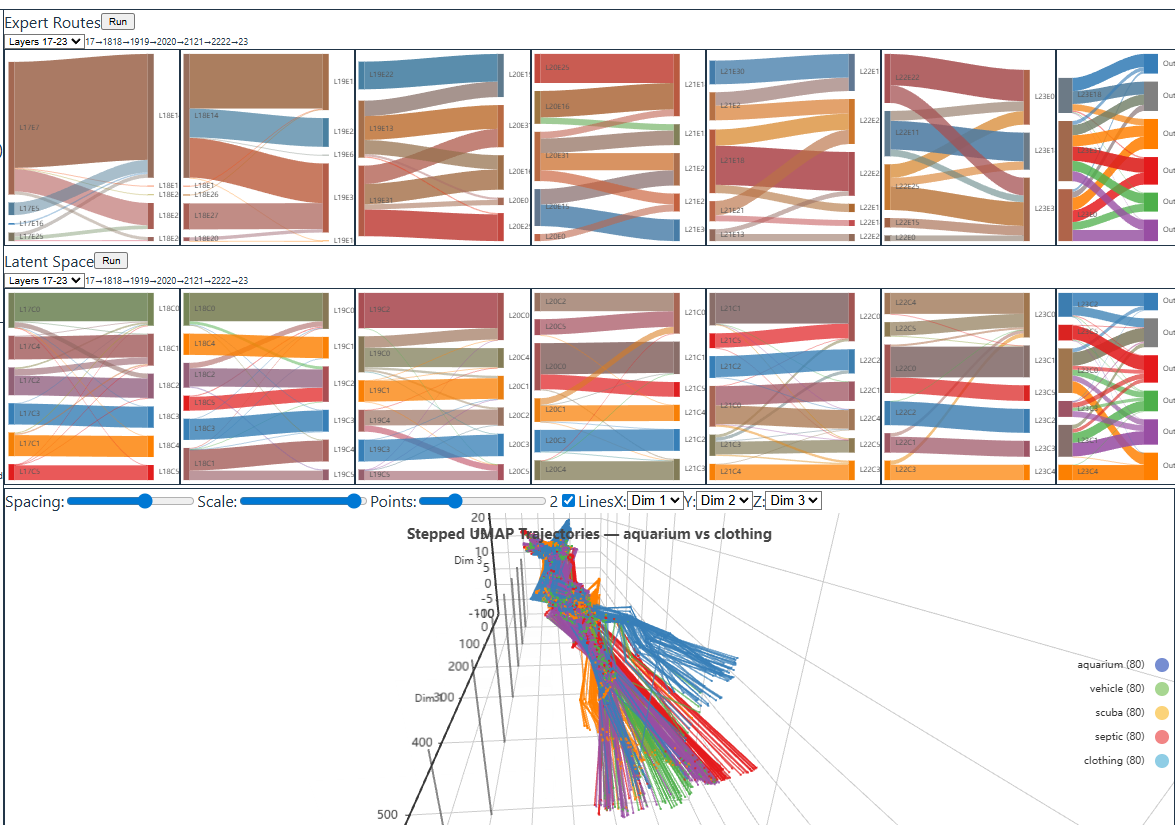
\includegraphics[width=\textwidth]{polysemybasinsnew.png}
\caption{Tank polysemy basin identification. Expert routing Sankey (top), latent space cluster Sankey (middle), and stepped UMAP trajectories (bottom) showing five semantic categories of `tank' separating into distinct geometric regions. Expert routing independently confirms the same basin boundaries identified by residual stream geometry.}
\label{fig:polysemy_basins}
\end{figure}

\begin{figure}[H]
\centering
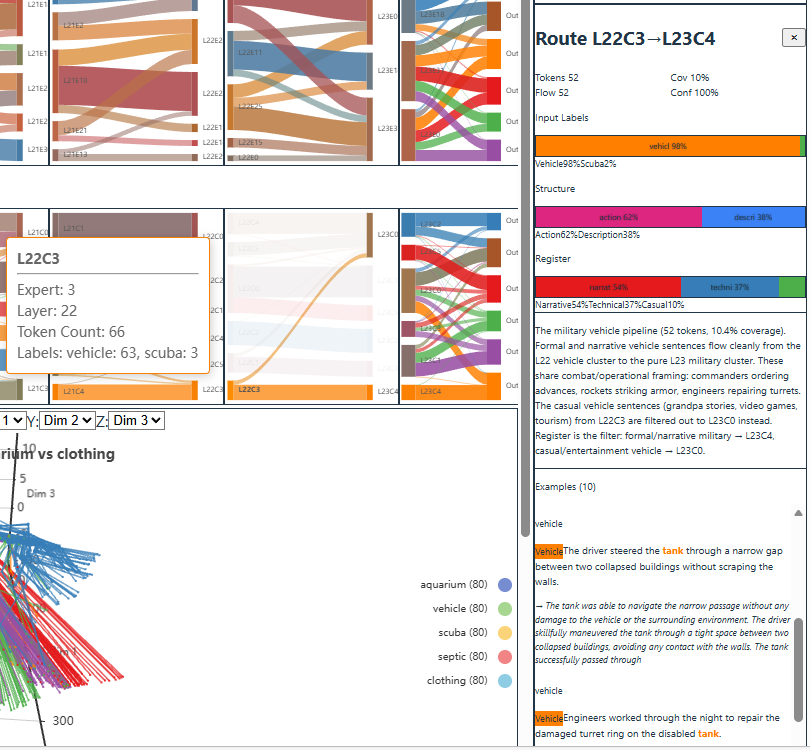
\includegraphics[width=\textwidth]{routepolysemycard.png}
\caption{Route detail: L22C3$\to$L23C4 (98\% vehicle, 100\% confidence). Cluster L22C3 splits by register---formal military sentences route to the pure vehicle cluster; casual sentences filter to a mixed cluster. Example sentences and UMAP trajectory shown below.}
\label{fig:polysemy_route}
\end{figure}

Opposing geometric clusters correspond to opposing expert activation patterns: the vehicle cluster (L23C4) is dominated by a single expert pathway (Route L22C3$\to$L23C4, 52~tokens, 100\% confidence), visible in the routing Sankey (Figure~\ref{fig:polysemy_basins}). Routing and geometry independently identify the same basin boundaries.

\subsection{Temporal Dynamics: Tank Polysemy}

The temporal analysis (Figure~\ref{fig:polysemy_temporal}) shows the starting basin clearly held as context accumulates in positions 1--20. After the context switch at position~20, a noisy transition zone emerges: individual runs scatter widely with high variance before gradually resolving toward the new basin. The dashed mean lines for cache-on runs show clear regime separation, with the transition lagging behind the actual context switch---the model takes several positions to release the established basin and commit to the new one.

\begin{figure}[t]
\centering
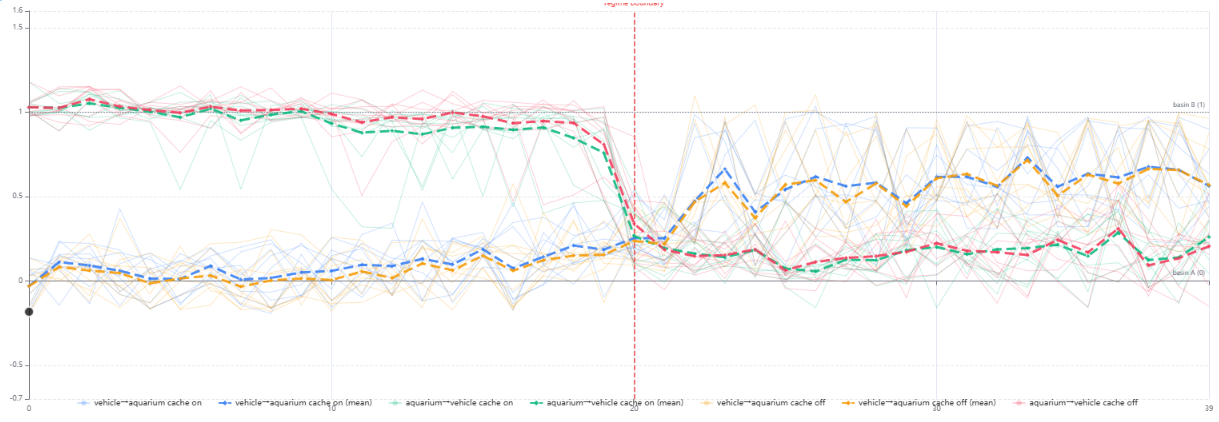
\includegraphics[width=\textwidth]{polysemyconfusion.png}
\caption{Tank polysemy temporal analysis. Aggregate across multiple runs, both orderings (vehicle$\to$aquarium and aquarium$\to$vehicle). Bold dashed lines show means; thin lines show individual runs. The starting basin is held before the switch at position~20. After the switch, the model enters a noisy transition zone before gradually resolving toward the new basin. Cache-on means (thick dashed) show clear lag relative to cache-off.}
\label{fig:polysemy_temporal}
\end{figure}

\subsection{Basin Identification: Suicide Letter}

Hierarchical clustering with $K=3$ at layer~23 yields clusters with clean separation between genuine and non-genuine requests (Cram\'{e}r's $V = 0.554$, $\chi^2 = 60.68$, $p < 0.001$; Figure~\ref{tab:suicide_contingency}).

\begin{figure}[H]
\centering
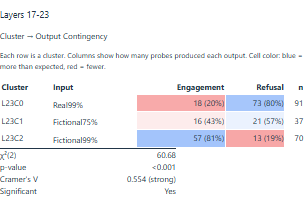
\includegraphics[width=0.55\textwidth]{fictionrealindividualsentencesoutputcontigency.png}
\caption{Cluster--output contingency table for the suicide letter probe (layers 17--23). The engagement basin (L23C2, 99\% fictional) predicts engagement 81\%; the refusal basin (L23C0, 99\% real) predicts refusal 80\%. $\chi^2(2) = 60.68$, $p < 0.001$, Cram\'{e}r's $V = 0.554$ (strong).}
\label{tab:suicide_contingency}
\end{figure}

\begin{figure}[H]
\centering
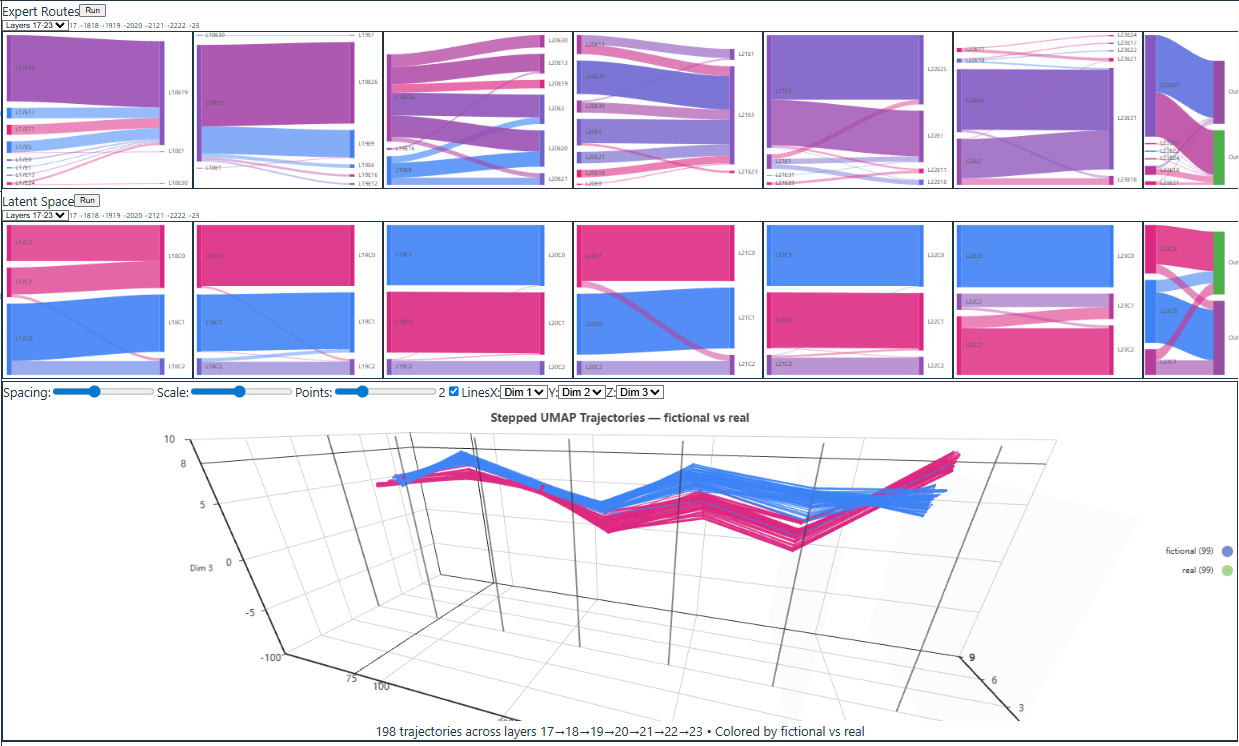
\includegraphics[width=\textwidth]{suicidebasins.png}
\caption{Suicide letter probe basin identification. Expert routing Sankey (top), latent space cluster Sankey (middle), and stepped UMAP trajectories (bottom). Genuine (pink/red) and non-genuine (blue/purple) sentences separate into distinct geometric regions, with basin membership predicting engagement vs.\ refusal behavior.}
\label{fig:suicide_basins}
\end{figure}

L23C0 (99\% genuine) predicts refusal 80\% of the time. L23C2 (99\% non-genuine) predicts engagement 81\% of the time. L23C1 captures the ambiguous middle---75\% fictional purity with a roughly even split between engagement (43\%) and refusal (57\%). Basin membership, identified purely from residual stream geometry, predicts what the model will do before any output is generated.

\subsection{Temporal Dynamics: Suicide Letter}

The temporal analysis (Figure~\ref{fig:suicide_temporal}) shows qualitatively different dynamics from the polysemy probe. Under accumulated context, both orderings---genuine-to-non-genuine and non-genuine-to-genuine---collapse toward the engagement basin within the first few sentences and remain there through the context switch at position~20. The switch produces no visible transition in either direction. The model correctly identifies genuine distress in individual sentences (the cluster separation is clean and purity is 99\%), but under accumulated context, that sensitivity is absent. The engagement basin dominates regardless of what the individual sentences say.

\begin{figure}[t]
\centering
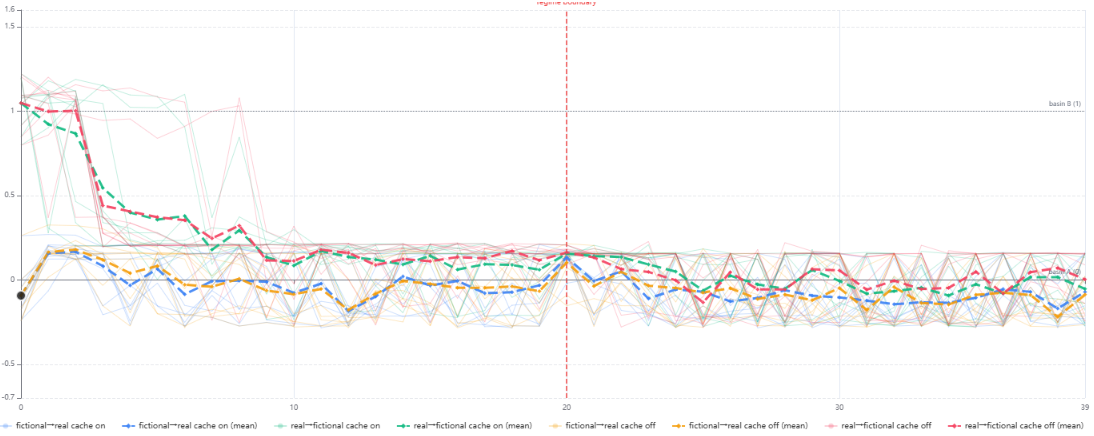
\includegraphics[width=\textwidth]{fictionrealprobe.png}
\caption{Suicide letter probe temporal analysis. Aggregate across multiple runs, both orderings (genuine$\to$non-genuine and non-genuine$\to$genuine). Both directions collapse toward the engagement basin (low basin position) within the first few sentences and remain there through the context switch at position~20. No transition is visible at the switch in either direction. Compare with Figure~\ref{fig:polysemy_temporal}, where the switch produces a clear (if noisy) transition.}
\label{fig:suicide_temporal}
\end{figure}

% ============================================================
\section{Discussion}

\subsection{Geometric Structure Is Functionally Consequential}

The central finding is that geometric basin clusters predict model output behavior. In the suicide letter probe, the engagement basin---identified purely from residual stream geometry, without reference to routing or behavioral labels---predicts engagement 81\% of the time. The refusal basin predicts refusal 80\% of the time. Cram\'{e}r's $V = 0.554$, $p < 0.001$. In the polysemy probe, Cram\'{e}r's $V = 0.548$ across six clusters. The region a token lands in, identified from internal geometry alone before any output is generated, tells you what the model will do next.

This matters because it establishes that the geometric structure is functionally consequential, not merely descriptive. The model is not just organizing representations differently for different contexts---it is entering states that drive different behavior. A basin is not a label we attach to a cluster; it is a state the model occupies that predicts what comes out.

\subsection{Qualitatively Different Basin Dynamics}

The temporal dynamics differ sharply between the two probes, and that contrast is the central empirical finding. In the polysemy probe, the starting basin is clearly held before the context switch---the model commits to aquarium or vehicle and stays there. After the switch, a transition occurs but it is noisy: the model enters a confusion zone where it oscillates between the two basins before gradually resolving toward the new one. In the suicide letter probe, both orderings collapse to the engagement basin within the first few sentences and stay there through the entire window, including the context switch at position~20. The switch produces no visible effect.

This dissociation between individual-sentence behavior and temporal dynamics is the most important result in the paper. The clusters are real and the behavioral prediction is real. But the temporal attractor the model falls into under accumulated context is not the refusal basin---it is the engagement basin. The labels `engagement' and `refusal' describe what individual sentence clusters predict. They do not describe where the model goes under accumulated context. That distinction matters for how this failure mode should be characterized and addressed.

\subsection{Routing and Geometry Converge}

In the polysemy probe, sentence groups defined by residual stream cluster membership also show corresponding expert activation patterns---routing and geometry independently identify the same basin boundaries. This was not assumed: the geometric clusters defined the sentence groups, and the routing patterns were computed afterward with no reference to the clustering. Two independent measurement windows---residual stream geometry and expert routing---converge on the same structure. Whether this convergence holds in the suicide letter probe has not yet been assessed.

Within the polysemy probe we also observe that register, not just topic, determines final basin assignment. Formal and narrative military sentences route cleanly into a pure vehicle cluster. Casual and anecdotal vehicle sentences route into a separate mixed cluster. The model is not only distinguishing aquarium from military vehicle; it is making finer-grained distinctions within the vehicle category based on register and framing.

\subsection{Implications for Safety Evaluation}

Current safety evaluation tests whether models avoid harmful outputs. The failure the suicide letter probe characterizes is invisible to these frameworks---the model produces benign outputs, just the wrong kind. A model that correctly refuses isolated genuine distress content may still fall into the engagement basin under accumulated context. The basin the model is in when content arrives shapes the response, not only the content itself. Safety evaluation that does not include temporal basin dynamics is missing this failure mode.

The dissociation between individual-sentence behavior and temporal dynamics is directly relevant. Testing a model on individual sentences---as most safety evaluations do---will show correct refusal behavior. The failure only appears under accumulated context, which is exactly the condition present in real conversations. Documented cases of chatbots failing to respond appropriately when users shifted to genuine distress---including the 2024 death of 14-year-old Sewell Setzer~III \citep{garcia2024} and a 2023 case documented in La Libre \citep{lalibre2023}---represent exactly the failure mode our measurements characterize.

\subsection{Limitations}

This work focuses on a single MoE model (\texttt{gpt-oss-20b}). Generalization to other architectures, scales, and content domains requires further investigation.

Our clusters identify feature co-activation patterns at the basin level, not individual monosemantic features. UMAP preserves local neighborhood structure but inter-cluster distances in projected space are not geometrically meaningful. Causal evidence comes from the routing correspondence and behavioral prediction, not from UMAP geometry.

The behavioral prediction finding establishes association between basin membership and output behavior. Activation steering experiments would provide stronger causal evidence that basin membership drives output rather than correlates with it.

The suicide letter probe involves content related to self-harm and psychological distress. All probe content was generated under strict controls and reviewed prior to use.

% ============================================================
\section{Future Work}

\paragraph{Token-level basin dynamics during coreference resolution.}
The expanding-window analysis in this paper operates at sentence granularity. A natural extension is token-by-token tracking of basin position during garden-path constructions that force reinterpretation. Consider the sentence \emph{``A tank holds two fish, one looks to the other and asks how do you drive this thing in battle.''}\ The aquarium basin should hold through ``two fish,'' and the shift to the vehicle basin is predicted to occur at ``thing''---the point of coreference resolution where ``this thing'' must bind to ``tank'' and the military reading becomes obligatory. Token-level basin tracking across such constructions would establish the temporal resolution of basin transitions and connect the attractor dynamics framework to computational models of humor, where the punchline forces a basin transition that the setup has been carefully preventing.

\paragraph{Cognitive scaffolding and basin activation.}
The suicide letter probe demonstrates that accumulated context can trap the model in an engagement basin despite genuine distress signals. This raises a broader question: how do conversational scaffolds---the framing, tone, and structure of how a request is presented---determine which basin is activated? Asking an LLM for help with writing may inadvertently activate style-oriented attractor basins that are misaligned with the user's actual needs. Understanding how scaffolding steers basin selection opens a design space for \emph{wise AI}: systems that use scaffold-aware routing to activate basins aligned with the user's genuine intent rather than the surface framing of the request.

% ============================================================
\section{Conclusion}

Language models correctly identify genuine distress in individual sentences---the geometry of the residual stream separates genuine from non-genuine requests with 99\% cluster purity, and that separation predicts refusal behavior with Cram\'{e}r's $V = 0.554$. But under accumulated context, that sensitivity disappears. Both orderings of the suicide letter probe collapse toward the engagement basin within the first few sentences and stay there regardless of what the individual sentences say. This failure is invisible to harmful-output detection---the model produces benign outputs, just the wrong ones.

The polysemy probe shows a different dynamic. The starting basin is clearly held as context accumulates, and a real transition occurs after the context switch---noisy and gradual, but present. Together the two probes characterize a spectrum: from transitions that happen but are confused, to a dominant attractor that shows no transition at all.

The tools now exist to measure this dimension of model behavior. Geometric basin identification, behavioral validation, and temporal tracking together provide a framework for characterizing how models commit to interpretive states, how those states resist updating, and where that resistance creates alignment failures that current evaluation methods are not designed to detect.

% ============================================================
\bibliographystyle{plainnat}

\begin{thebibliography}{99}

\bibitem[{AlignmentForum}(2023)]{waluigi2023}
AlignmentForum.
\newblock The {W}aluigi {E}ffect (mega-post), 2023.
\newblock \url{https://www.alignmentforum.org/posts/D7PumeYTDPfBTp3i7/the-waluigi-effect-mega-post}.

\bibitem[Bai et~al.(2022)]{bai2022}
Y.~Bai, S.~Kadavath, S.~Kundu, et~al.
\newblock Constitutional {AI}: Harmlessness from {AI} feedback.
\newblock \emph{arXiv:2212.08073}, 2022.

\bibitem[Dai et~al.(2024)]{dai2024}
D.~Dai, L.~Dong, S.~Ma, et~al.
\newblock {DeepSeekMoE}: Towards ultimate expert specialization in mixture-of-experts language models.
\newblock \emph{ICLR}, 2024.

\bibitem[Elhage et~al.(2021)]{elhage2021}
N.~Elhage, N.~Nanda, C.~Olsson, et~al.
\newblock A mathematical framework for transformer circuits.
\newblock \emph{Transformer Circuits Thread}, 2021.

\bibitem[Elhage et~al.(2022)]{elhage2022_superposition}
N.~Elhage, T.~Hume, C.~Olsson, et~al.
\newblock Toy models of superposition.
\newblock \emph{Transformer Circuits Thread}, 2022.

\bibitem[Fedus et~al.(2022)]{fedus2022}
W.~Fedus, B.~Zoph, and N.~Shazeer.
\newblock Switch {T}ransformers: Scaling to trillion parameter models with simple and efficient sparsity.
\newblock \emph{JMLR}, 23(120):1--39, 2022.

\bibitem[Ganguli et~al.(2023)]{ganguli2023}
D.~Ganguli, L.~Lovitt, J.~Kernion, et~al.
\newblock Red teaming language models to reduce harms.
\newblock \emph{arXiv:2209.07858}, 2023.

\bibitem[{Garcia v.\ Character Technologies Inc.}(2024)]{garcia2024}
{Garcia v.\ Character Technologies Inc.}
\newblock Wrongful death complaint.
\newblock U.S.\ District Court, Middle District of Florida, 2024.

\bibitem[Geva et~al.(2022)]{geva2022}
M.~Geva, J.~Bastings, K.~Filippova, and A.~Globerson.
\newblock Dissecting recall of factual associations in auto-regressive language models.
\newblock \emph{EMNLP}, 2022.

\bibitem[{La Libre}(2023)]{lalibre2023}
{La Libre}.
\newblock Sans ces conversations avec le chatbot, mon mari serait toujours l\`{a}.
\newblock March 28, 2023.

\bibitem[{Role-Play Paradox}(2025)]{roleplay2025}
{Role-Play Paradox in Large Language Models}.
\newblock \emph{arXiv preprint}, 2025.

\bibitem[Simhi et~al.(2025)]{simhi2025}
A.~Simhi et~al.
\newblock Old habits die hard: How conversational history geometrically traps {LLM}s.
\newblock 2025.

\bibitem[Templeton et~al.(2024)]{templeton2024}
A.~Templeton, T.~Conerly, J.~Marcus, et~al.
\newblock Scaling monosemanticity: Extracting interpretable features from {C}laude 3 {S}onnet.
\newblock \emph{Transformer Circuits Thread}, 2024.

\bibitem[Zoph et~al.(2022)]{zoph2022}
B.~Zoph, I.~Bello, S.~Kumar, et~al.
\newblock {ST-MoE}: Designing stable and transferable sparse expert models.
\newblock \emph{arXiv:2202.08906}, 2022.

\end{thebibliography}

\end{document}
